% Created by tikzDevice version 0.12 on 2018-10-26 14:06:55
% !TEX encoding = UTF-8 Unicode
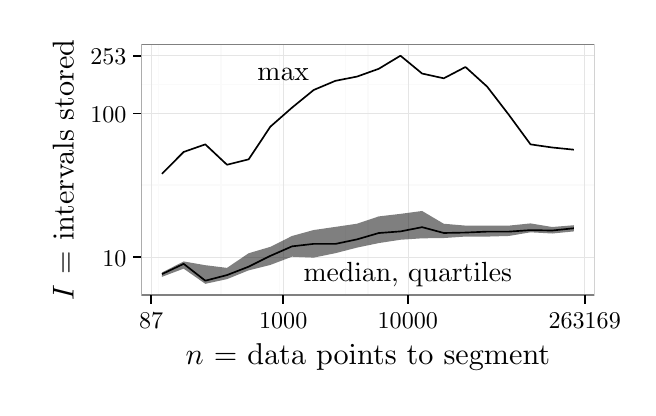
\begin{tikzpicture}[x=1pt,y=1pt]
\definecolor{fillColor}{RGB}{255,255,255}
\path[use as bounding box,fill=fillColor,fill opacity=0.00] (0,0) rectangle (216.81,130.09);
\begin{scope}
\path[clip] (  0.00,  0.00) rectangle (216.81,130.09);
\definecolor{drawColor}{RGB}{255,255,255}
\definecolor{fillColor}{RGB}{255,255,255}

\path[draw=drawColor,line width= 0.6pt,line join=round,line cap=round,fill=fillColor] ( -0.00,  0.00) rectangle (216.81,130.09);
\end{scope}
\begin{scope}
\path[clip] ( 41.08, 33.41) rectangle (204.81,124.09);
\definecolor{fillColor}{RGB}{255,255,255}

\path[fill=fillColor] ( 41.08, 33.41) rectangle (204.81,124.09);
\definecolor{drawColor}{gray}{0.98}

\path[draw=drawColor,line width= 0.6pt,line join=round] ( 41.08, 73.12) --
	(204.81, 73.12);

\path[draw=drawColor,line width= 0.6pt,line join=round] ( 41.08,109.51) --
	(204.81,109.51);

\path[draw=drawColor,line width= 0.6pt,line join=round] ( 47.33, 33.41) --
	( 47.33,124.09);

\path[draw=drawColor,line width= 0.6pt,line join=round] ( 69.83, 33.41) --
	( 69.83,124.09);

\path[draw=drawColor,line width= 0.6pt,line join=round] (114.85, 33.41) --
	(114.85,124.09);

\path[draw=drawColor,line width= 0.6pt,line join=round] ( 90.98, 33.41) --
	( 90.98,124.09);

\path[draw=drawColor,line width= 0.6pt,line join=round] (122.95, 33.41) --
	(122.95,124.09);
\definecolor{drawColor}{gray}{0.90}

\path[draw=drawColor,line width= 0.2pt,line join=round] ( 41.08, 47.19) --
	(204.81, 47.19);

\path[draw=drawColor,line width= 0.2pt,line join=round] ( 41.08, 99.06) --
	(204.81, 99.06);

\path[draw=drawColor,line width= 0.2pt,line join=round] ( 41.08,119.96) --
	(204.81,119.96);

\path[draw=drawColor,line width= 0.2pt,line join=round] ( 92.34, 33.41) --
	( 92.34,124.09);

\path[draw=drawColor,line width= 0.2pt,line join=round] (137.36, 33.41) --
	(137.36,124.09);

\path[draw=drawColor,line width= 0.2pt,line join=round] ( 44.61, 33.41) --
	( 44.61,124.09);

\path[draw=drawColor,line width= 0.2pt,line join=round] (201.28, 33.41) --
	(201.28,124.09);
\definecolor{drawColor}{RGB}{0,0,0}

\node[text=drawColor,anchor=base,inner sep=0pt, outer sep=0pt, scale=  1.00] at ( 92.34,110.83) {max};

\node[text=drawColor,anchor=base,inner sep=0pt, outer sep=0pt, scale=  1.00] at (137.36, 38.38) {median, quartiles};

\path[draw=drawColor,line width= 0.6pt,line join=round] ( 48.52, 77.26) --
	( 56.36, 85.18) --
	( 64.19, 87.92) --
	( 72.02, 80.56) --
	( 79.86, 82.52) --
	( 87.69, 94.31) --
	( 95.53,101.20) --
	(103.36,107.58) --
	(111.19,110.88) --
	(119.03,112.42) --
	(126.86,115.23) --
	(134.70,119.96) --
	(142.53,113.51) --
	(150.36,111.79) --
	(158.20,115.88) --
	(166.03,108.78) --
	(173.87, 98.60) --
	(181.70, 87.92) --
	(189.53, 86.79) --
	(197.37, 86.00);
\definecolor{fillColor}{RGB}{0,0,0}

\path[fill=fillColor,fill opacity=0.50] ( 48.52, 41.61) --
	( 56.36, 45.62) --
	( 64.19, 44.26) --
	( 72.02, 43.29) --
	( 79.86, 48.58) --
	( 87.69, 50.89) --
	( 95.53, 54.82) --
	(103.36, 56.97) --
	(111.19, 58.10) --
	(119.03, 59.25) --
	(126.86, 61.89) --
	(134.70, 62.81) --
	(142.53, 63.85) --
	(150.36, 59.23) --
	(158.20, 58.57) --
	(166.03, 58.52) --
	(173.87, 58.56) --
	(181.70, 59.36) --
	(189.53, 58.06) --
	(197.37, 58.70) --
	(197.37, 56.47) --
	(189.53, 55.71) --
	(181.70, 56.15) --
	(173.87, 54.82) --
	(166.03, 54.60) --
	(158.20, 54.61) --
	(150.36, 54.07) --
	(142.53, 53.97) --
	(134.70, 53.45) --
	(126.86, 52.25) --
	(119.03, 50.62) --
	(111.19, 48.60) --
	(103.36, 47.00) --
	( 95.53, 47.33) --
	( 87.69, 44.36) --
	( 79.86, 42.40) --
	( 72.02, 39.22) --
	( 64.19, 37.53) --
	( 56.36, 43.01) --
	( 48.52, 40.05) --
	cycle;

\path[draw=drawColor,line width= 0.6pt,line join=round] ( 48.52, 41.04) --
	( 56.36, 44.75) --
	( 64.19, 38.66) --
	( 72.02, 40.69) --
	( 79.86, 43.73) --
	( 87.69, 47.63) --
	( 95.53, 51.07) --
	(103.36, 51.97) --
	(111.19, 51.95) --
	(119.03, 53.60) --
	(126.86, 55.88) --
	(134.70, 56.47) --
	(142.53, 58.00) --
	(150.36, 55.90) --
	(158.20, 56.05) --
	(166.03, 56.39) --
	(173.87, 56.39) --
	(181.70, 56.94) --
	(189.53, 56.79) --
	(197.37, 57.61);
\definecolor{drawColor}{gray}{0.50}

\path[draw=drawColor,line width= 0.6pt,line join=round,line cap=round] ( 41.08, 33.41) rectangle (204.81,124.09);
\end{scope}
\begin{scope}
\path[clip] (  0.00,  0.00) rectangle (216.81,130.09);
\definecolor{drawColor}{RGB}{0,0,0}

\node[text=drawColor,anchor=base east,inner sep=0pt, outer sep=0pt, scale=  0.87] at ( 35.68, 43.90) {10};

\node[text=drawColor,anchor=base east,inner sep=0pt, outer sep=0pt, scale=  0.87] at ( 35.68, 95.77) {100};

\node[text=drawColor,anchor=base east,inner sep=0pt, outer sep=0pt, scale=  0.87] at ( 35.68,116.67) {253};
\end{scope}
\begin{scope}
\path[clip] (  0.00,  0.00) rectangle (216.81,130.09);
\definecolor{drawColor}{RGB}{0,0,0}

\path[draw=drawColor,line width= 0.6pt,line join=round] ( 38.08, 47.19) --
	( 41.08, 47.19);

\path[draw=drawColor,line width= 0.6pt,line join=round] ( 38.08, 99.06) --
	( 41.08, 99.06);

\path[draw=drawColor,line width= 0.6pt,line join=round] ( 38.08,119.96) --
	( 41.08,119.96);
\end{scope}
\begin{scope}
\path[clip] (  0.00,  0.00) rectangle (216.81,130.09);
\definecolor{drawColor}{RGB}{0,0,0}

\path[draw=drawColor,line width= 0.6pt,line join=round] ( 92.34, 30.41) --
	( 92.34, 33.41);

\path[draw=drawColor,line width= 0.6pt,line join=round] (137.36, 30.41) --
	(137.36, 33.41);

\path[draw=drawColor,line width= 0.6pt,line join=round] ( 44.61, 30.41) --
	( 44.61, 33.41);

\path[draw=drawColor,line width= 0.6pt,line join=round] (201.28, 30.41) --
	(201.28, 33.41);
\end{scope}
\begin{scope}
\path[clip] (  0.00,  0.00) rectangle (216.81,130.09);
\definecolor{drawColor}{RGB}{0,0,0}

\node[text=drawColor,anchor=base,inner sep=0pt, outer sep=0pt, scale=  0.87] at ( 92.34, 21.43) {1000};

\node[text=drawColor,anchor=base,inner sep=0pt, outer sep=0pt, scale=  0.87] at (137.36, 21.43) {10000};

\node[text=drawColor,anchor=base,inner sep=0pt, outer sep=0pt, scale=  0.87] at ( 44.61, 21.43) {87};

\node[text=drawColor,anchor=base,inner sep=0pt, outer sep=0pt, scale=  0.87] at (201.28, 21.43) {263169};
\end{scope}
\begin{scope}
\path[clip] (  0.00,  0.00) rectangle (216.81,130.09);
\definecolor{drawColor}{RGB}{0,0,0}

\node[text=drawColor,anchor=base,inner sep=0pt, outer sep=0pt, scale=  1.09] at (122.95,  8.40) {$n$ = data points to segment};
\end{scope}
\begin{scope}
\path[clip] (  0.00,  0.00) rectangle (216.81,130.09);
\definecolor{drawColor}{RGB}{0,0,0}

\node[text=drawColor,rotate= 90.00,anchor=base,inner sep=0pt, outer sep=0pt, scale=  1.09] at ( 16.63, 78.75) {$I$ = intervals stored};
\end{scope}
\end{tikzpicture}
